\section{Technical implementation and details}

\subsection{FIDO2}

As already briefly introduced in \autoref{subsec:fido_alliance}, the \gls{fido}2 project is a joint efforts of the \gls{w3c} and the \gls{fido} alliance. It consists of the JavaScript standard, the \wa{}, and the \gls{ctap}. The \wa{} is standardized and managed by the \gls{w3c}, while the \gls{ctap} is authored by the \gls{fido} alliance. However, the \gls{fido} alliance also initially developed the \wa{} under the name \gls{fido} 2.0 before officially handing it over to the \gls{w3c}.\footcites[See][254]{Schwartz2018}[See][3]{FormalVerificationWebAuthn}

\begin{figure}[hbt]
	\centering
	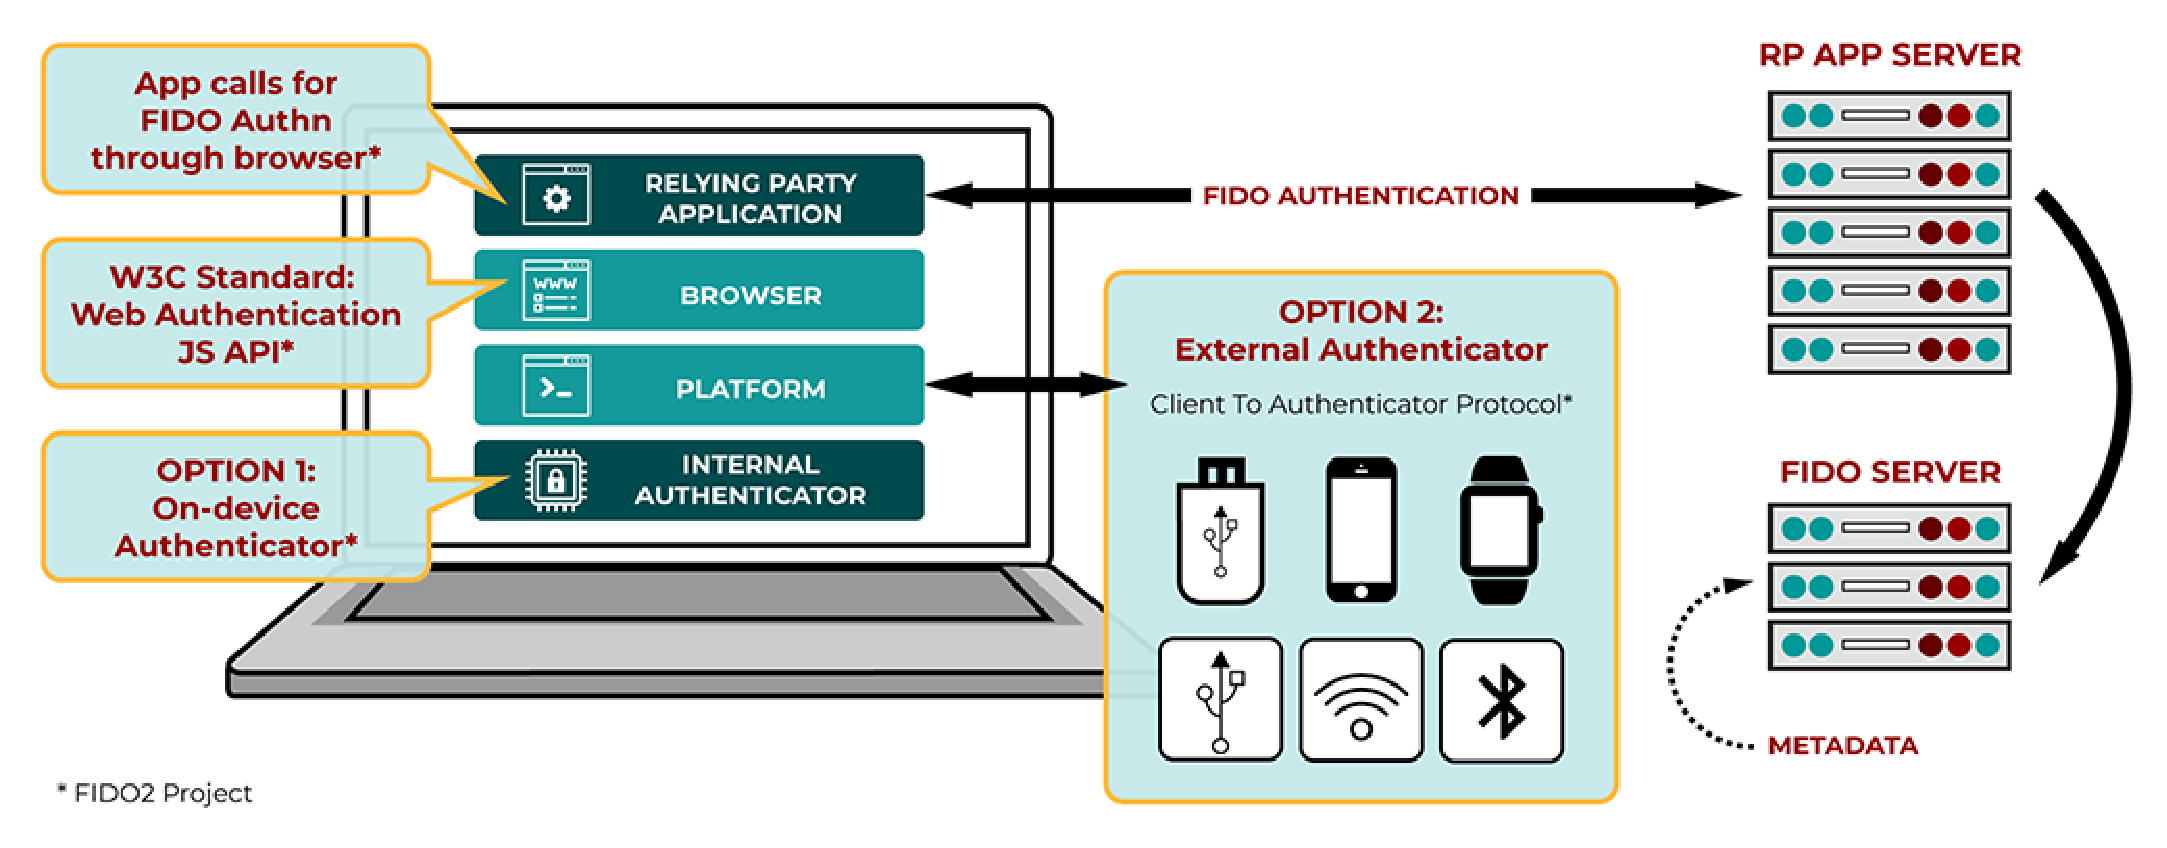
\includegraphics[width=\textwidth]{pics/FIDO2-Graphic-v2.eps}
	\caption[\gls{fido}2 architecture overview]{\gls{fido}2 architecture overview\footnotemark}
	\label{fig:fido2_architecture}
\end{figure}
\footnotetext{Source: https://fidoalliance.org/specifications/, last access on 09/14/2019}

\autoref{fig:fido2_architecture} shows the overview of the \gls{fido}2 project. A noteworthy change is the possibility to use either a \textit{roaming}, i.e., external authenticator or an authenticator that is built into the device.

\subsection{Client to Authenticator Protocol 2}

The \glsfirst{ctap} 2 is based on the \gls{u2f} protocol version 1.2 and defines three parts:

\begin{enumerate}
	\item the authenticator \gls{api}
	\item message encoding
	\item transport-specifc binding
\end{enumerate}

The key methods of the authenticator \gls{api} are explained in more detail below. Message encoding describes the process of encoding the corresponding message in a binary encoding called \gls{cbor} that is suitable for, e.g., the transport over \gls{ble}, because plain text string and \gls{json} objects might be too big. The transport-specific bindings define the required transformation and bindings in order to comply with the transport protocol specifications.\footcites[See][4--5]{ctap2}

An important difference between \gls{ctap}2 and the preceding standard \gls{u2f} is the fact that \gls{ctap}2 describes only the communication between the client, i.e., web browser and the authenticator, as opposed to \gls{u2f} where the standard also defines the JavaScript \gls{api} in order to communicate with the authenticator. \autoref{fig:ctap_vs_u2f} shows this architectural difference.\footcites[See][51]{kim-new-way-fido}[See][254]{Schwartz2018}

\begin{figure}[hbt]
	\centering
	\includesvg[width=\textwidth,pretex=\relscale{0.8}]{pics/svg/ctap_vs_u2f}
	\caption[Architectural differences of \gls{u2f} and \gls{ctap}2]{Architectural differences of \gls{u2f} and \gls{ctap}2\footnotemark}
	\label{fig:ctap_vs_u2f}
\end{figure}
\footcitetexts[Source: diagram by author, based on][4]{u2f-overview}[][Chapter 6]{w3c}

\subsubsection{Registration}

The registration calls the method \textit{authenticatorMakeCredential}. The input parameters are identical to the ones defined in the higher level \wa{} and are further explained in \autoref{subsec:wa}. Upon reception of the required data, the authenticator first checks if the \textit{excludeList} if a credential ID is listed that is already registered on the authenticator. This prevents that a user registers multiple accounts. If the user verification or presence option is passed, the authenticator has to ensure a legitimate user is present. Upon successful user verification the authenticator generates a new credential key-pair for the specified algorithm.

After that, the authenticator generates the attestation object consisting of  the authentication data, which contain the hash of the \gls{rp} ID, a counter, flags if the user has been verified, and the public key with its unique credential ID. Besides that, the authenticator also sends the attestation statement

\subsubsection{Authentication}

\subsubsection{Factory reset}

As the \gls{uaf} protocol, but in contrast to the \gls{u2f} specification, the \gls{ctap} does define a method to completely factory reset the authenticator in order to de-register every user account on it. To avoid accidental deletion of all user accounts, the protocol specifies that the authenticator may ask for user confirmation. However, it is not possible to delete a specific user account. 

\subsection{Web Authentication API}
\label{subsec:wa}

The \wa{} is backwards compatible to the \gls{u2f} compatible, thus making every security token that is usable for \gls{u2f} compatible with the \wa, too.